
\documentclass{article}
\def\pgfsysdriver{pgfsys-tex4ht.def}
\usepackage{pgf}
\usepackage{amsmath}
\usepackage{tikz}
\usetikzlibrary{arrows,automata}
\tikzstyle{every node}=[font=\Large]
\usepackage[latin1]{inputenc}
\begin{document}
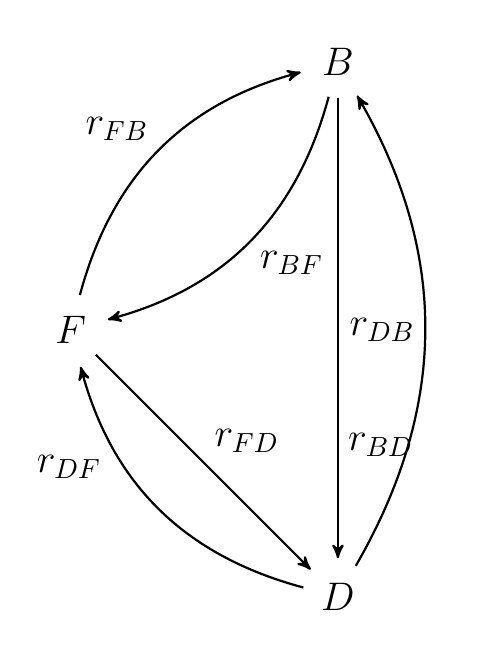
\begin{tikzpicture}[->,>=stealth',shorten >=1pt,auto,node distance=4.8cm,
                    thick,font=\Large]
  \tikzstyle{every state}=[fill=white,draw=none,text=black]

  \node[state] 	       (F)                    {$F$};
  \node[state]         (B) [above right of=F] {$B$};
  \node[state]         (D) [below right of=F] {$D$};

  \path (F) edge [bend left]             node {$r_{FB}$} (B) 
            edge             node {$r_{FD}$} (D) 
        (B) edge [bend left]	 	 node {$r_{BF}$} (F) 
            edge 		 node [near end] {$r_{BD}$} (D)
        (D) edge [bend left]             node [near end] {$r_{DF}$} (F)
            edge [bend right]  		node [pos=0.5] {$r_{DB}$} (B);
\end{tikzpicture}

\end{document}
